\documentclass[12pt,twoside]{article}

% Things that are not loaded by the package, though these might be
% generally useful.
\usepackage{natbib}
\usepackage{graphicx}
\setcounter{secnumdepth}{0}

\usepackage{amsthm}
\newcommand{\E}{\mathrm{E}}
\newcommand{\Var}{\mathrm{Var}}
\newcommand{\Cov}{\mathrm{Cov}}

% Load the package first - should sort everything out...
\usepackage{suppmat}

% ...and then we add some metadata
\titleprefix{Supplemental Material}
\runninghead{PCA in comparative analyses}
\title{Comparative analysis of principal components can be misleading}
\author{Josef C. Uyeda, Daniel S. Caetano, \& Matthew W. Pennell}
\address{Department of Biological Sciences \& Institute for Bioinformatics
an Evolutionary Studies, University of Idaho}
\emailaddress{\email{josef.uyeda@gmail.com}}
\date{}

\begin{document}

\maketitle

\section{Appendix: Equivalency between Ornstein-Uhlenbeck and Accelerating Change models}

In our paper, we investigate the scenario in which the individual traits have each evolved under a different model. To simulate the data, we drew values for the exponential rate parameter $r$ of the accelerating/decelerating change \citep[ACDC;][]{Blomberg2003} model for each trait from a normal distribution with mean 0. We claim that when $r$ is positive, the ACDC model generates traits with a structure equivalent to those produced by a single optimum Ornstein-Uhlenbeck \citep[OU;][]{Hansen1997} model. To our knowledge, this has not been previously demonstrated in the literature. \citet{SlaterFossil} suggested that these two models were equivalent for ultrametric trees: ``Looking at extant taxa only, the outcome of [a process with accelerating rates] is very similar to an OU process, as both tend to erase phylogenetic signal'' [p. 3940], though they did not provide any proof.\bigskip

\noindent \emph{Conjecture.} A single optimum OU process produces identical covariance matrices to those produced by the AC model when i) the tree is ultrametric and ii) the trait is assumed to be at the optimum at the root of the tree.

\begin{proof}

Consider a bifurcating tree of depth $T$ with two terminal taxa $i$ and $j$ that are sampled at the present and share a common ancestor at time $t_{ij}$ where $t_{ij} < T$. A trait $Y$ is measured for both $i$ and $j$.\bigskip

\par{\textsc{Ornstein-Uhlenbeck process}}\\
First, assume that $Y$ has evolved according to an Ornstein-Uhlenbeck (OU) process 
\begin{equation}
dY = -\alpha(Y - \theta)dt + \sigma dW
\end{equation}
where $\theta$ is the optimum trait value, $\alpha$ is the strength of the pull towards $\theta$, and $\sigma$ is the rate of the Brownian diffusion process $dW$ \citep{Hansen1997}. Also assume that the process began at the optimum, such that $Y(t=0) = \theta$. The expected value for $Y_i$ and $Y_j$ is equal to the root state. The expected variance for both $Y_i$ and $Y_j$ is given by \citet{Hansen1997}:
\begin{equation}\label{eq:var-ou}
\Var[Y_i] = \Var[Y_j] = \frac{\sigma^2}{2\alpha}(1-e^{-2\alpha T})
\end{equation}
The expected covariance between lineages $Y_i$ and $Y_j$ is given by
\begin{equation}
\Cov[Y_i, Y_j] = \frac{\sigma^2}{2\alpha}e^{-2 \alpha (T-t_{ij})}(1-e^{-2\alpha t_{ij}}) 
\end{equation}
The correlation between $Y_i$ and $Y_j$, $\rho[Y_i, Y_j]$, is defined as
\[\rho[Y_i, Y_j] = \frac{\Cov[Y_i, Y_j]}{\sqrt{\Var[Y_i]\Var[Y_j]}}\]
Under an OU process, $\rho[Y_i, Y_j]$ is
\begin{equation}\label{eq:rho-ou}
\rho[Y_i, Y_j] = \frac{\frac{\sigma^2}{2\alpha}e^{-2 \alpha (T-t_{ij})}(1-e^{-2\alpha t_{ij}})}{\frac{\sigma^2}{2\alpha}(1-e^{-2\alpha T})}
\end{equation}
With some algebra, it is straightforward to reduce Equation \ref{eq:rho-ou} to
%% This is t_{ij} in equation (5), correct?
\begin{equation}
\frac{1-e^{2\alpha t_{ij}}}
{1-e^{2\alpha T}}
\end{equation}\bigskip

\par{\textsc{Accelerating Change Model}}\\
Next, assume that $Y$ has evolved according to the Accelerating Change (AC) model, which describes a Brownian motion process in which the rate of diffusion $\sigma^2$ changes as function of time
\begin{equation}
dY(t)=\sigma(t)dW. 
\end{equation}
Specifically, we consider the functional form of $\sigma^2(t)$ to be
\[\sigma^2 (t) = \sigma^2_0 e^{rt}\]
where $r$ is constrained to be positive \citep{Blomberg2003, SlaterFossil}. The expected value of the AC model is also equal to the root state. The expected variance for $Y_i$ and $Y_j$ is given by
\begin{equation}\label{eq:var-ac}
\Var[Y_i] = \Var[Y_j] = \int^T_0 \sigma^2_0 e^{rT} dt = \sigma^2_0 \left( \frac{e^{rT} - 1}{r} \right)
\end{equation}
\citep{Harmon2010} and the covariance is equal to
\begin{equation}
\Cov[Y_i,Y_j] = \int^{t_{ij}}_0 \sigma^2_0 e^{rt_{ij}} dt = \sigma^2_0 \left( \frac{e^{rt_{ij}} - 1}{r} \right)
\end{equation}
Under the AC model, $\rho[Y_i, Y_j]$ is
\begin{equation}\label{eq:rho-ac}
\rho[Y_i, Y_j] = \frac{\sigma^2_0 \left( \frac{e^{rt_{ij}} - 1}{r} \right)}{\sigma^2_0 \left( \frac{e^{rT} - 1}{r} \right)}
\end{equation}
Equation \ref{eq:rho-ac} can be easily reduced to
\begin{equation}
\frac{1-e^{rt_{ij}}}{1-e^{r T}}
\end{equation}\bigskip

\par{\textsc{Comparing the expectations under OU and AC}}\\
Comparing equations \ref{eq:rho-ou} and \ref{eq:rho-ac}, it is clear that the correlation between $Y_i$ and $Y_j$ under the OU model is equal to that of the AC model
\begin{equation}
\frac{1-e^{2\alpha t_{ij}}}
{1-e^{2\alpha T}} = \frac{1-e^{r t_{ij}}}{1-e^{r T}}
\end{equation}
when $\alpha = \text{0.5}r$. For every value of $\alpha$ there is a value of $r$ that can produce an identical correlation structure. Note that the values of $\sigma^2$ and $\sigma^2_0$ do not affect the correlation structure but do enter into the covariance structure. As $\Cov[Y_i, Y_j] = \Var[Y_i, Y_j]\rho[Y_i, Y_j]$ and the values of $\rho[Y_i, Y_j]$ are equivalent, we can set the variances of two models (given by Equations \ref{eq:var-ou} and \ref{eq:var-ac}) equal to one another
\begin{equation}\label{eq:var}
\frac{\sigma^2}{2\alpha}(1 - e^{-2\alpha T}) = \sigma^2_0 \left(\frac{e^{rT} - 1}{r} \right)
\end{equation}
and substitute $r$ for $2\alpha$
\[\frac{\sigma^2}{r}(1 - e^{-r T}) = \sigma^2_0 \left(\frac{e^{r T} - 1}{r} \right)\]
Reducing algebraically, it is easy to show that
\begin{equation}
\sigma^2 = \sigma^2_0 e^{rT}
\end{equation}
Therefore for any covariance matrix for $Y_i$ and $Y_j$, OU and AC are completely unidentifiable and the likelihoods for the two models will be identical.

\end{proof}

\noindent \emph{Notes.} The two variances $\Var[Y_i]$ and $\Var[Y_j]$ will only be equal to one another when the tree is ultrametric. If either $i$ or $j$ were not sampled at the present (e.g., if one was an extinct lineage), this proof for the non-identifiability of OU and AC does not hold and one can potentially distinguish these models \citep{SlaterFossil}.


\renewcommand\thefigure{S.\arabic{figure}}
\renewcommand\thetable{S.\arabic{table}}
\clearpage
\listoffigures

%% Figure S1.
\begin{figure}[p]
\centering
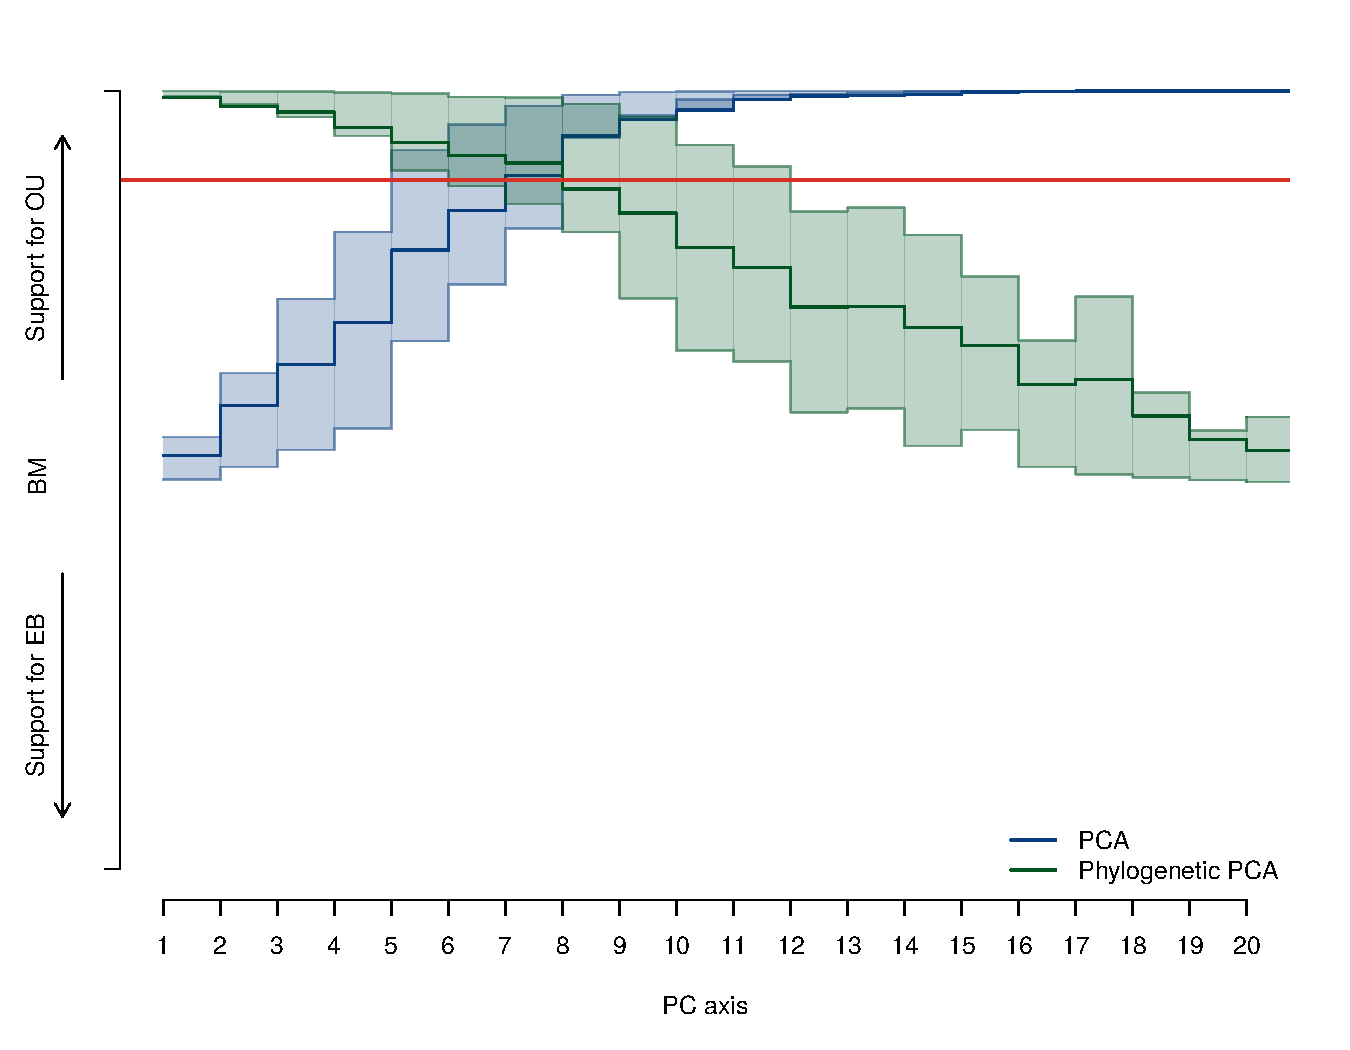
\includegraphics[scale=0.65]{./fig/uncor-ou-aic.pdf}
\caption[Model support when generating model is uncorrelated OU]{Distribution of support for BM, OU and EB models when the generating model is a uncorrelated multivariate OU model. Support for models were transformed into a linear scale by calculating an overall model support statistic: $AICw_{OU} - AICw_{EB}$. Thus high values support OU, low values support EB, and intermediate values near 0 indicate BM-like evolution. Models were fit to each replicated dataset for each of 20 different traits which were taken either from PC scores (blue line) or phylogenetic PC scores (green line). Shaded regions indicate the 25$^{th}$ and 75$^{th}$ quantiles of the model support statistic for 100 replicated datasets. The red line indicates the average model support statistic averaged over all 20 original trait variables. Note that standard PCA results in Akaike weights that are skewed toward EB for the first few PCs of standard PCA, while  and that later PCs subsequently favor OU models. By contrast, pPCA results in Akaike weights that are skewed toward stronger support for OU models relative to the original trait variables.}
\label{oufit}
\end{figure}

%% Figure S2.
\begin{figure}[p]
\centering
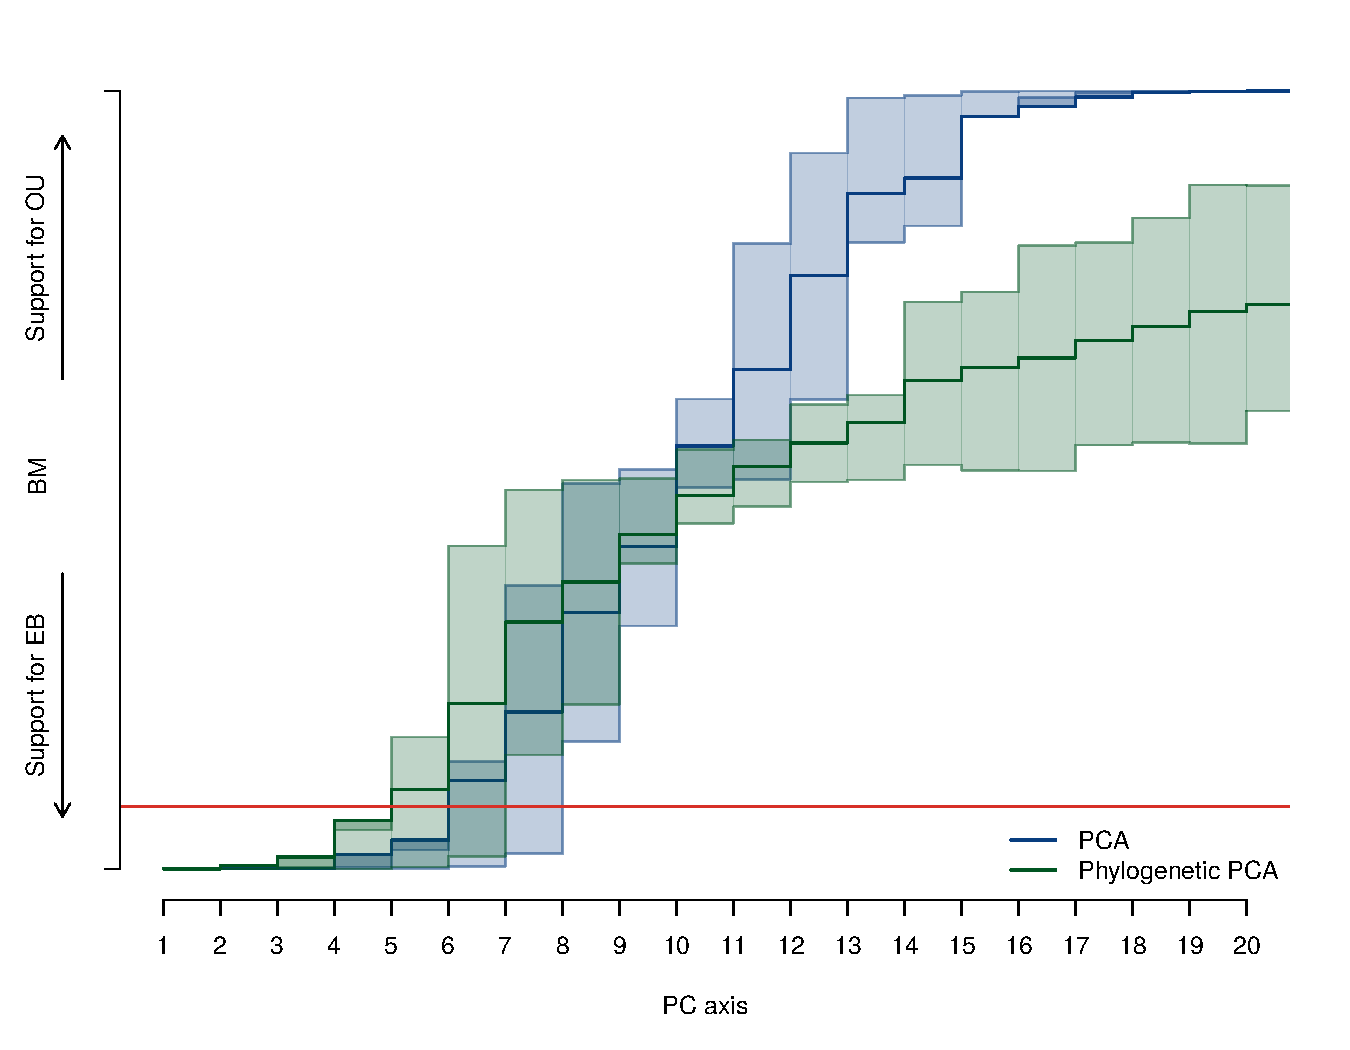
\includegraphics[scale=0.65]{./fig/uncor-eb-aic.pdf}
\caption[Model support when generating model is uncorrelated EB]{Distribution of support for BM, OU and EB models when the generating model is an uncorrelated multivariate EB model. Support for models were transformed into a linear scale by calculating an overall model support statistic: $AICw_{OU} - AICw_{EB}$. Thus high values support OU, low values support EB, and intermediate values near 0 indicate BM-like evolution. Models were fit to each replicated dataset for each of 20 different traits which were taken either from PC scores (blue line) or phylogenetic PC scores (green line). Shaded regions indicate the 25$^{th}$ and 75$^{th}$ quantiles of the model--support statistic for 100 replicated datasets. The red  line indicates the average model support statistic averaged over all 20 original trait variables. Note that both pPCA and PCA increase support for EB models for early PC axes.}
\label{aicweb}
\end{figure}

%% Figure S3.
\begin{figure}[p]
\centering
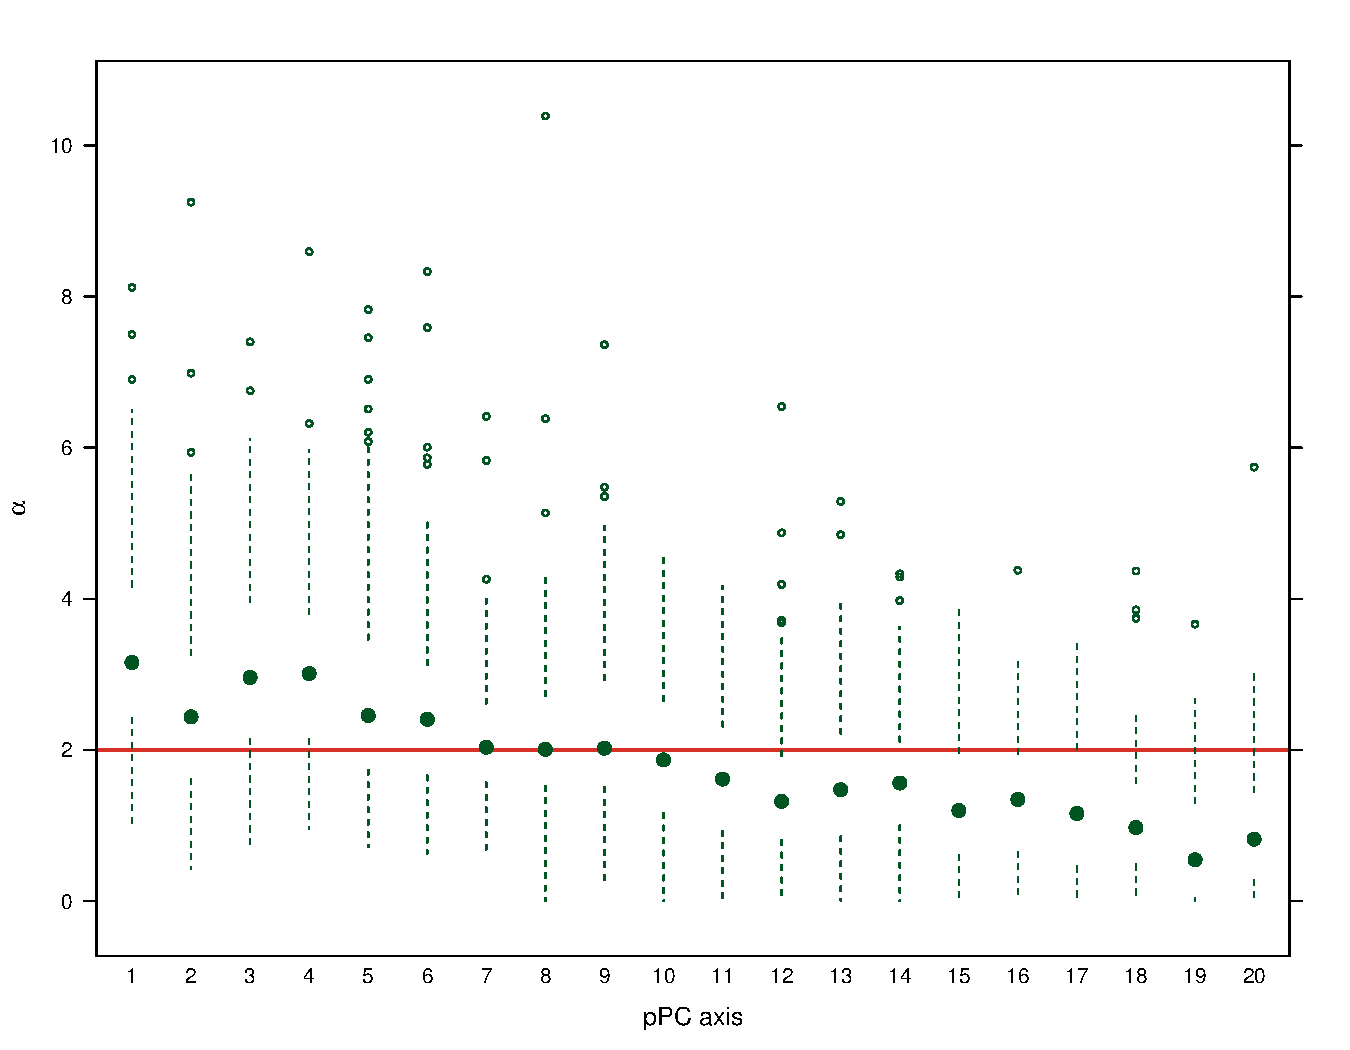
\includegraphics[scale=0.65]{fig/alpha-est-corr.pdf}
\caption[Estimates of the $\alpha$ parameter from phylogenetic PCA on correlated OU]{Estimated values of the $\alpha$ parameter from phylogenetic PCA when data is simulated under a correlated multivariate OU model. The simulating value $\alpha=$ 2 is depicted with the red line. The estimate of $\alpha$ is inflated in the first few pPC axes consistent with an exaggerated support for the OU model. In the last pPC axes, $\alpha$ is estimated to be very close to 0, such that the OU model is statistically indistinguishable from a BM model.}
\label{alpha-cor}
\end{figure}

%% Figure S4.
\begin{figure}[p]
\centering
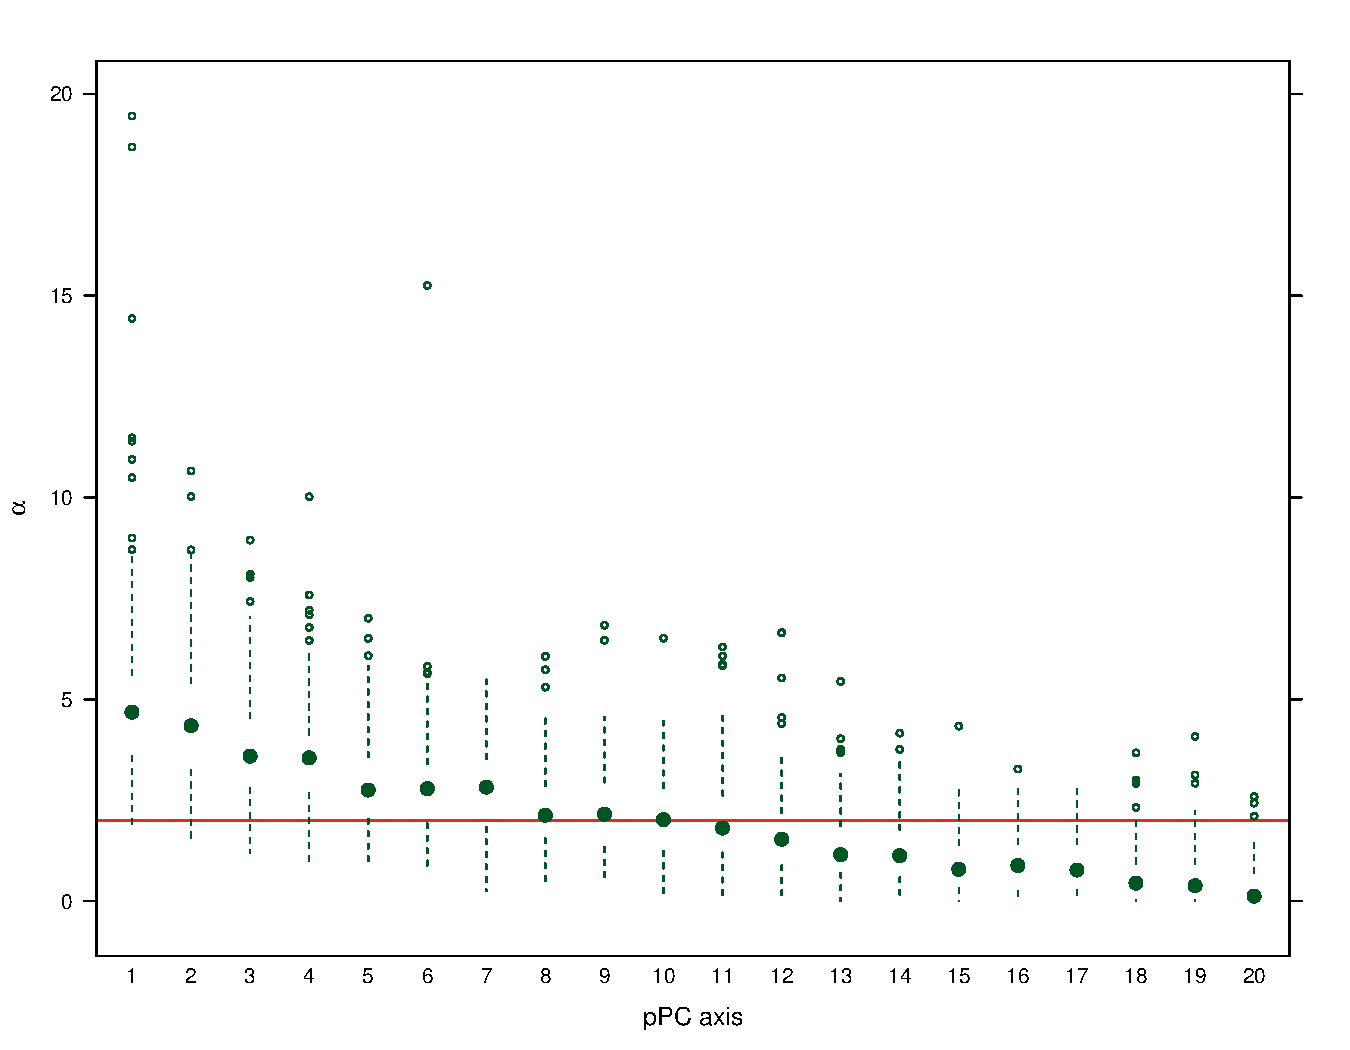
\includegraphics[scale=0.65]{fig/alpha-est-uncor.pdf}
\caption[Estimates of the $\alpha$ parameter from phylogenetic PCA on uncorrelated OU]{Estimated values of the $\alpha$ parameter from phylogenetic PCA when data is simulated under an uncorrelated multivariate OU model. The simulating value $\alpha=$ 2 is depicted with the red line. The estimate of $\alpha$ is inflated in the first few pPC axes consistent with an exaggerated support for the OU model. In the last pPC axes, $\alpha$ is estimated to be very close to 0, such that the OU model is statistically indistinguishable from a BM model.}
\label{alpha-uncor}
\end{figure}

%% Figure S5.
\begin{figure}[p]
\centering
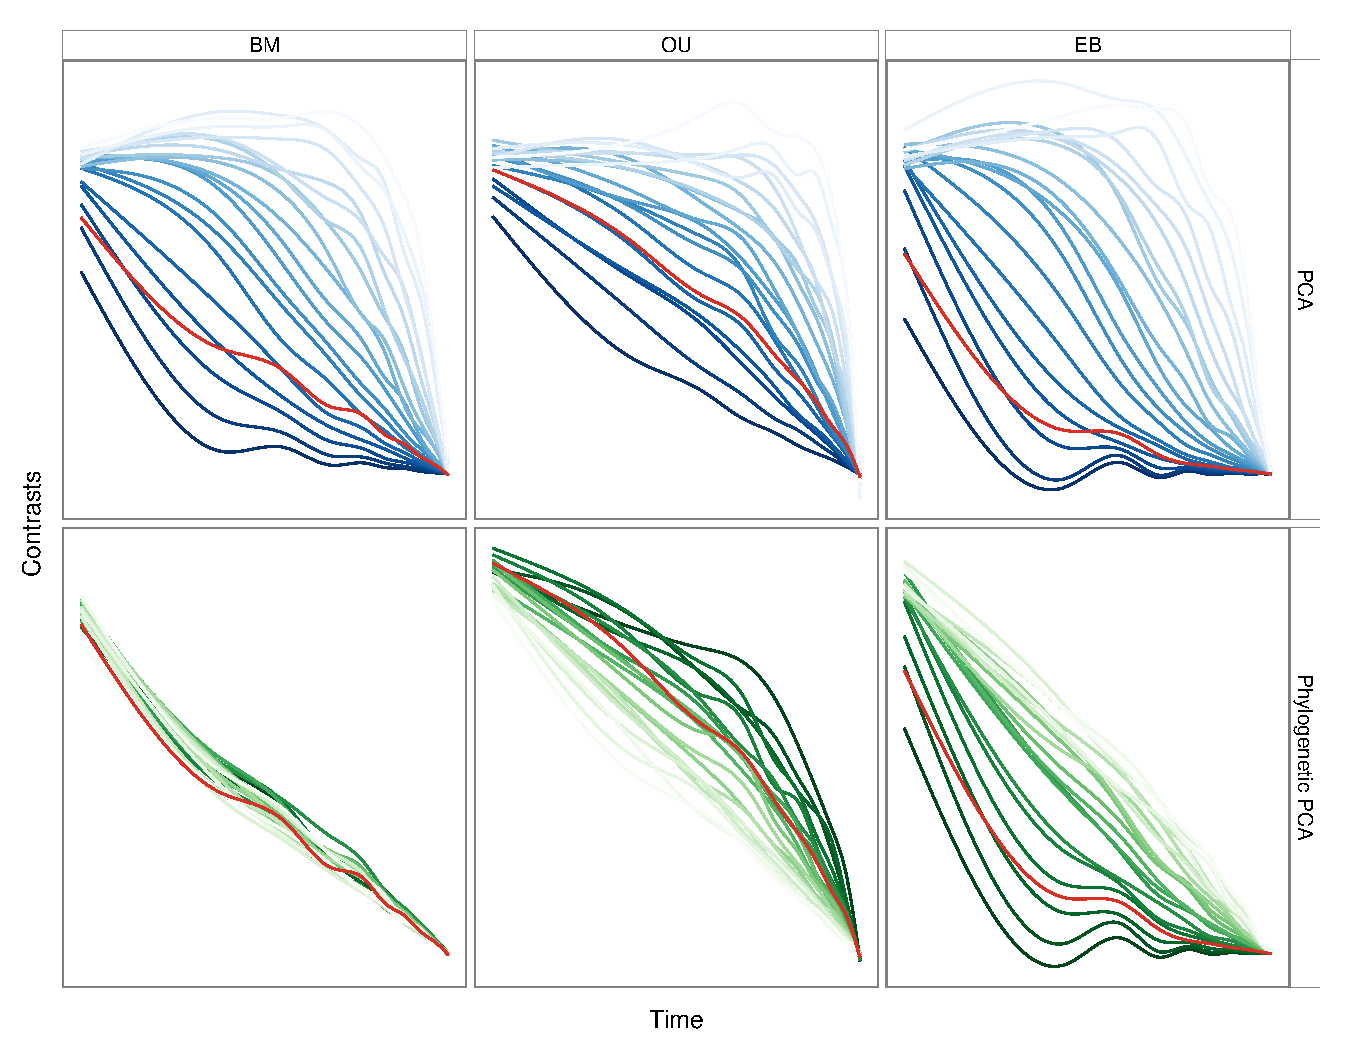
\includegraphics[scale=0.65]{./fig/dtt-2panel.pdf}
\caption[Disparity through time plots]{Disparity through time plots averaged across the 100 simulated datasets. The datasets were simulated under BM (left), OU (middle) or EB (right). The analyses were then performed on PC scores (top row) and pPC scores (bottom row). The average disparity through time of all 20 original trait variables is indicated by the red line. We fit a loess curve through the relative disparities for each trait/transformation/model combination. The plots are oriented so that the left side of each panel corresponds to the root of the phylogeny, with time increasing tipward to the right. The intensity of the colors are proportional to the ranking of the PC or pPC axes, stronger lines represent the first axes. As in Fig. 3, the first few axes from the PCA show a strong pattern of high disparity early in the clades' histories with the higher components showing seemingly higher disparity towards the present. Phylogenetic PCA corrects the distortion if the generating model is multivariate BM. However, if the generating model was not BM, the first few pPC axes tend to show an exaggerated pattern of disparity relative to the original traits.}
\label{dttplot}
\end{figure}

%% Figure S6.
\begin{figure}[p]
\centering
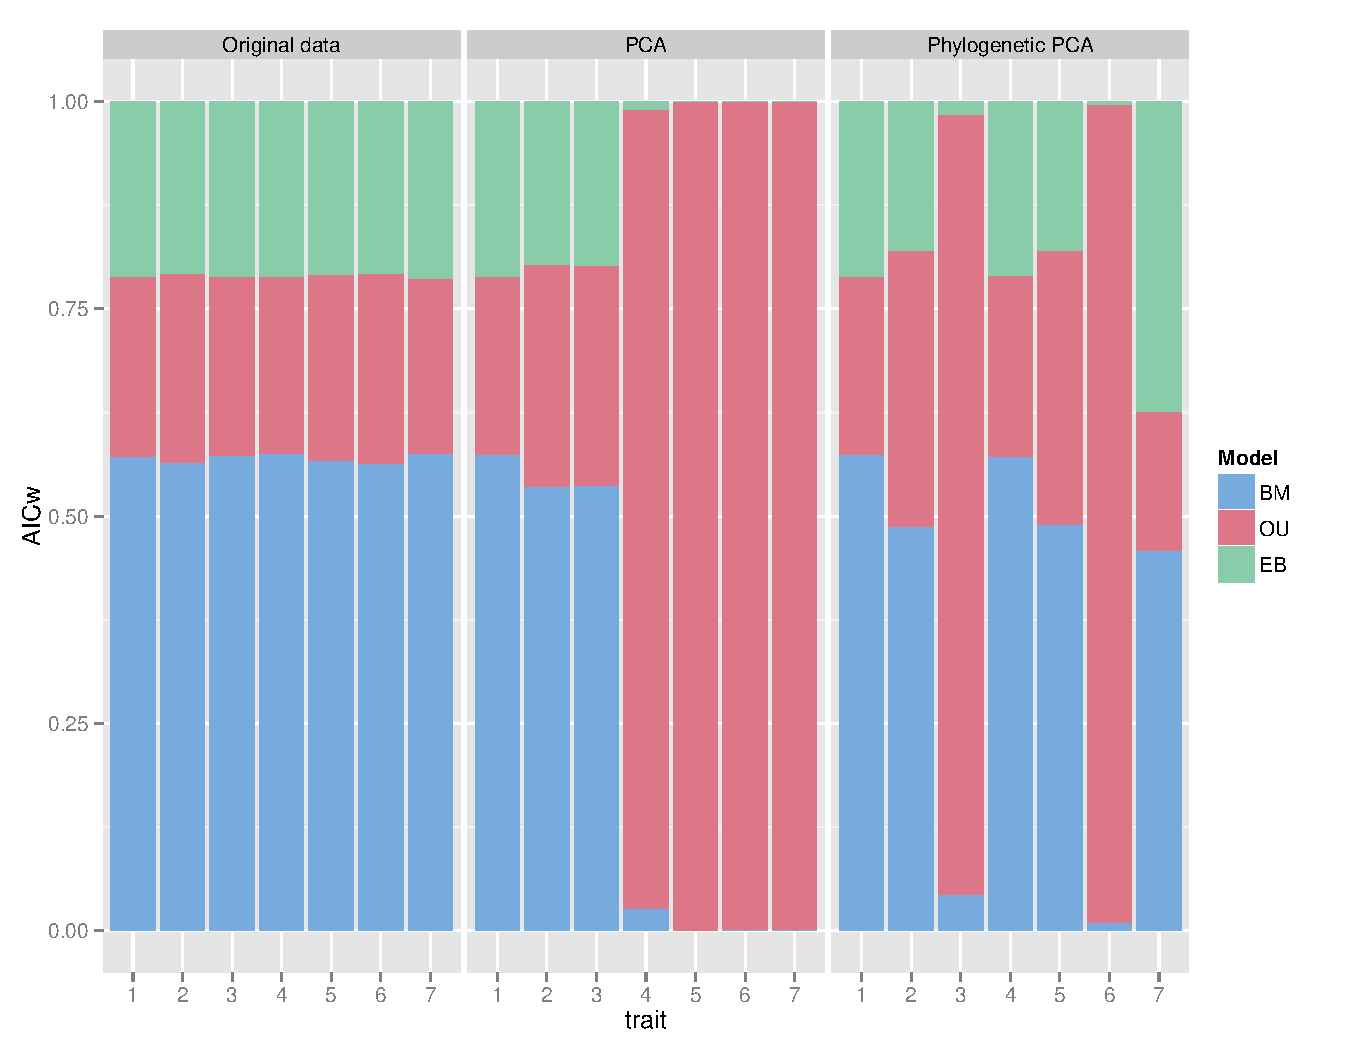
\includegraphics[scale=0.65]{fig/felidae_aicw.pdf}
\caption[Model support on the Felidae dataset]{Proportion of support for BM, OU and EB models for each of the traits/PC axes from the morphological dataset of Felidae species from \citet{Slater_2009} and \citet{sakamoto_2010}. Traits were log transformed prior to analysis. Note that all original traits and the first axes under standard and phylogenetic PCA show strong support for a BM model.}
\label{felidae.aicw}
\end{figure}

%% Figure S7.
\begin{figure}[p]
\centering
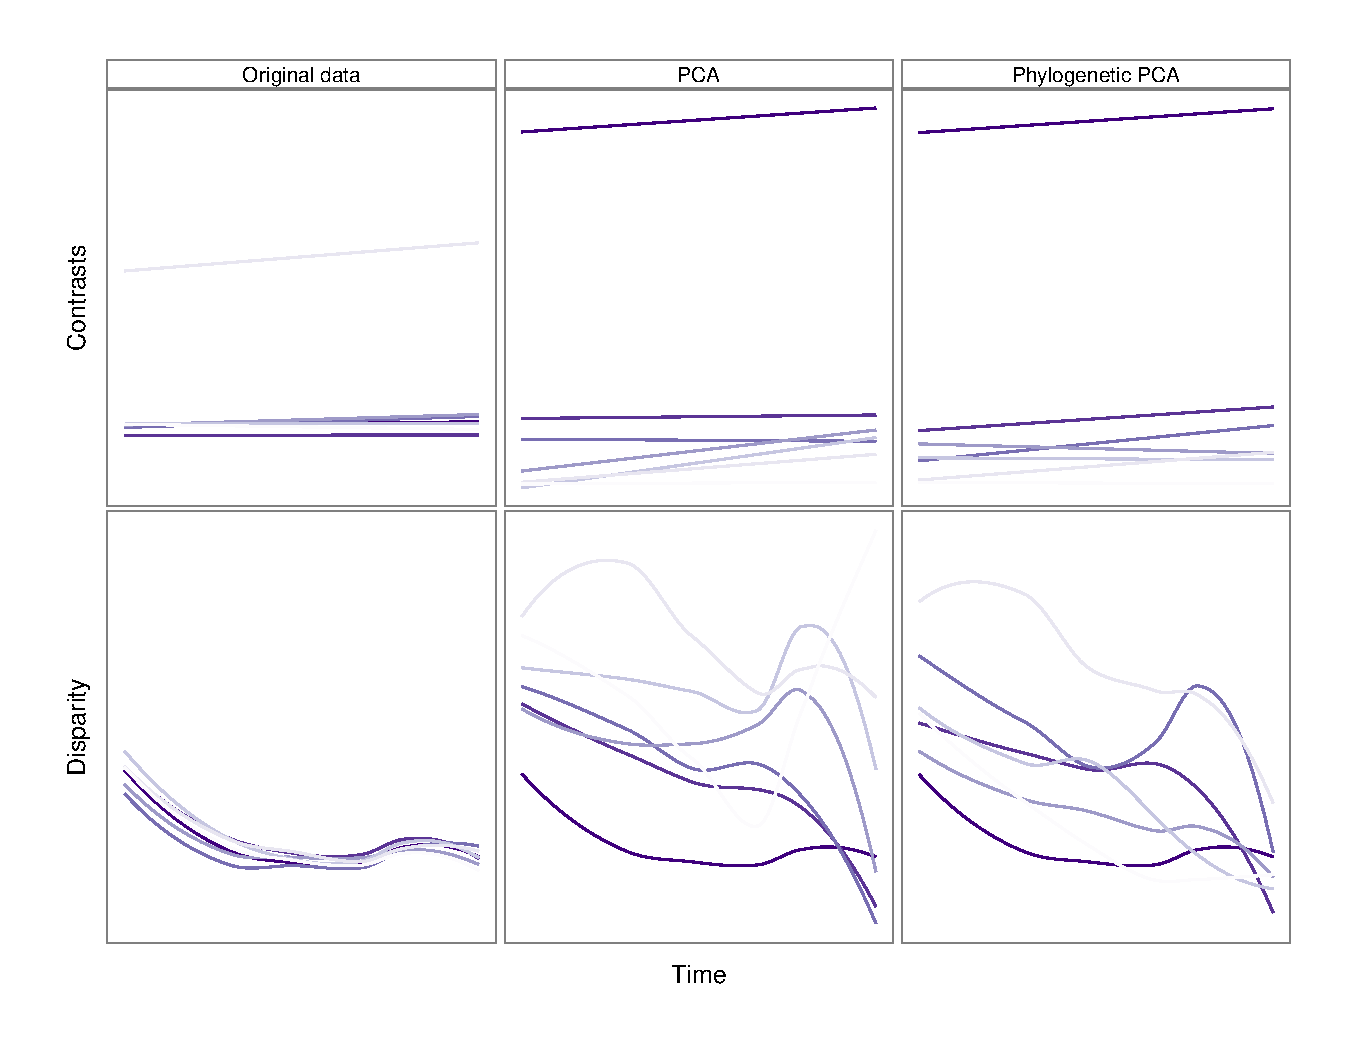
\includegraphics[scale=0.65]{fig/felidae_nh-dtt.pdf}
\caption[Node height test and disparity through time on the Felidae dataset]{Node height test and disparity through time plots for the morphological dataset of Felidae species. Each line represents a best--fit linear model (left) or loess curve fitted (right) to the original traits, PC or pPC scores. All traits were log transformed prior to analysis. The intensity of color is proportional to the ranking of the PC or pPC axes, stronger lines represent the first axes. Left panels show the relationship between the average phylogenetic independent contrasts and the height of the node. Red lines indicate the average value for the original trait values. Right panels show disparity through time plots. The plots are oriented so that the left side of each panel corresponds to the root of the phylogeny, with time increasing tipward to the right. Compare this highly correlated dataset with only 7 traits to the larger, less correlated dataset of \textit{Anolis} lizards (Figure \ref{anoles_nh}).}
\label{felidae.nh}
\end{figure}

%% Figure S8.
\begin{figure}[p]
\centering
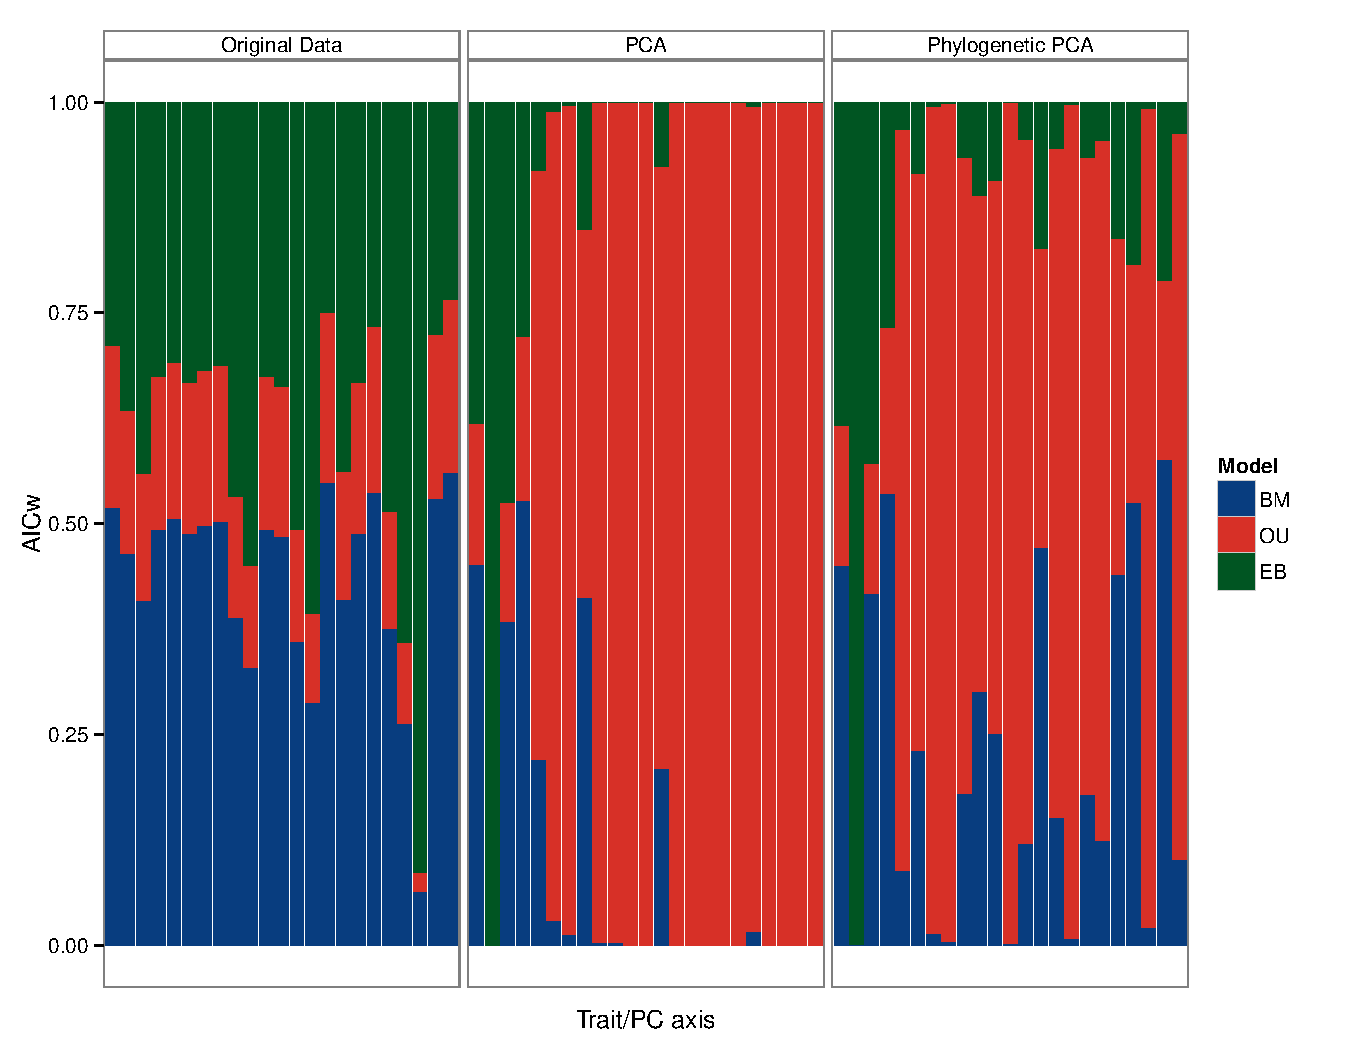
\includegraphics[scale=0.65]{./fig/anoles_aicw.pdf}
\caption[Model support on the \emph{Anolis} dataset]{Distribution of support for BM, OU and EB models for a 23--trait morphometric dataset taken from \citet{Mahler2010}. Support is measured in Akaike weights across all original trait variables (left), as well as standard PCA (middle) and pPCA (right). For both PCA and pPCA, support for the EB model appears to be concentrated in PCs 1-4, with a suggestive pattern of decreasing support across PCs 2-4. }
\label{anoles_aicw}
\end{figure}

%% Figure S9.
\begin{figure}[p]
\centering
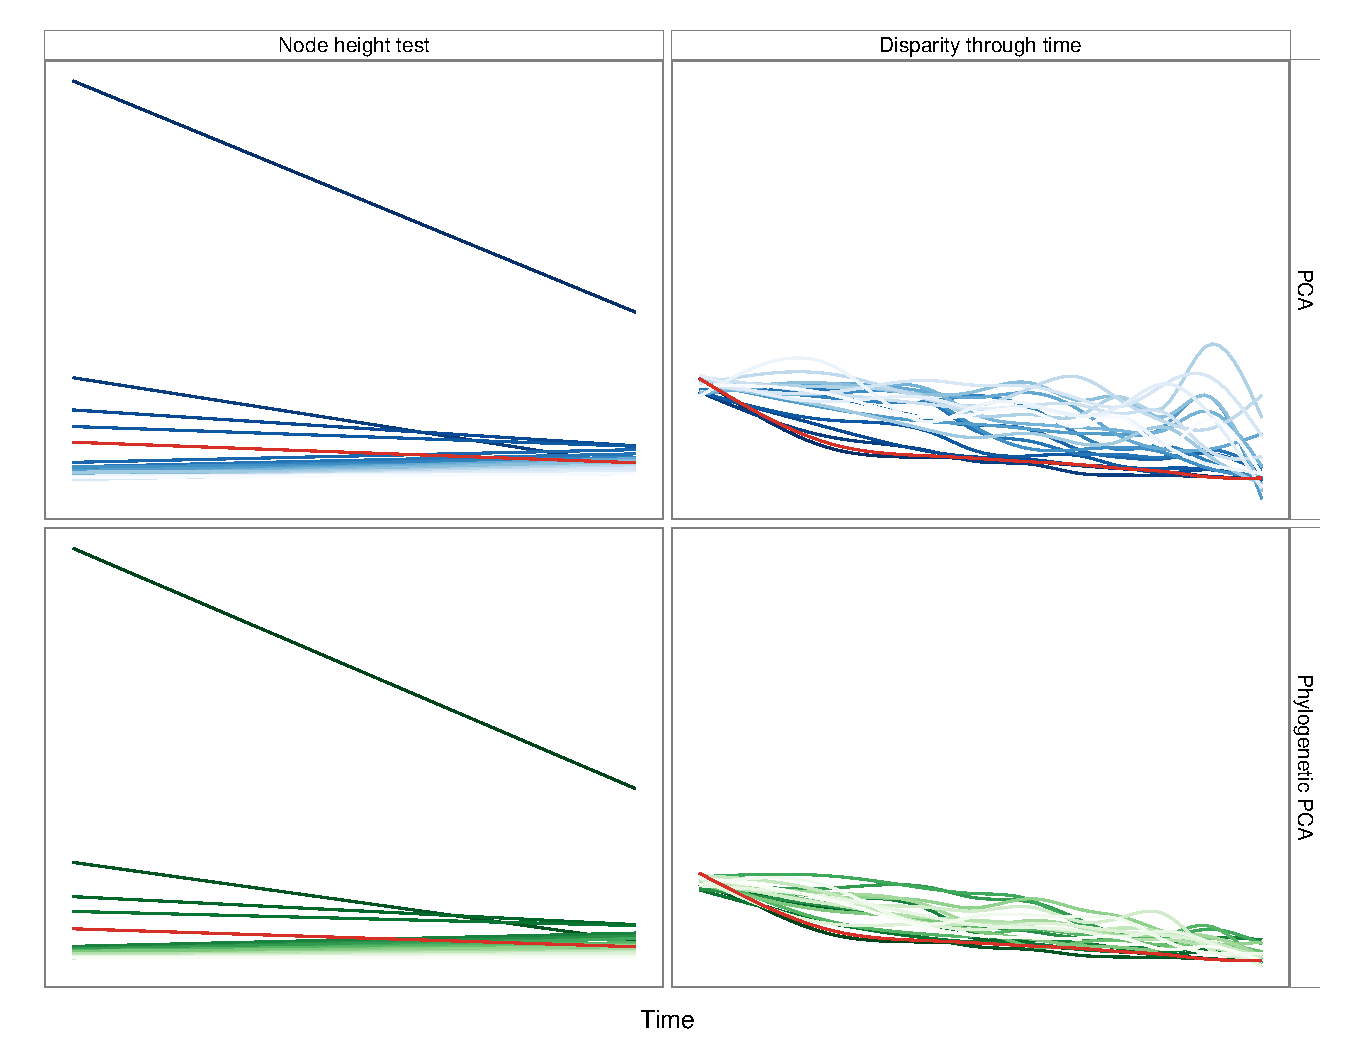
\includegraphics[scale=0.65]{./fig/anoles_nh-dtt.pdf}
\caption[Node height test and disparity through time on the \emph{Anolis} dataset]{Node height test and disparity through time plots for the morphological dataset of \textit{Anolis} lizards. Each line represents a best--fit linear model (left) or loess curve fitted (right) to the original traits, PC or pPC scores. All traits were log transformed prior to analysis. The intensity of color is proportional to the ranking of the PC or pPC axes, stronger lines represent the first axes. Left panels show the relationship between the average phylogenetic independent contrasts and the height of the node. Red lines indicate the average value for the original trait values. Right panels show disparity through time plots. The plots are oriented so that the left side of each panel corresponds to the root of the phylogeny, with time increasing tipward to the right. }
\label{anoles_nh}
\end{figure}


\clearpage
\bibliographystyle{sysbio}
\bibliography{phylopca.bib}

\end{document}
